\documentclass[10pt,a4paper,twocolumn,twoside]{article}
\usepackage[utf8]{inputenc}
\usepackage[catalan]{babel}
\usepackage{multicol}
\usepackage{graphicx}
\usepackage{fancyhdr}
\usepackage{times}
\usepackage{titlesec}
\usepackage{multirow}
\usepackage{lettrine}
\usepackage[top=2cm, bottom=1.5cm, left=2cm, right=2cm]{geometry}
\usepackage[figurename=Fig.,tablename=TAULA]{caption}
\PassOptionsToPackage{hyphens}{url}\usepackage{hyperref}
\usepackage{listings}

\lstset{
  breaklines=true,
  tabsize=2,
}

\captionsetup[table]{textfont=sc}

\titlespacing*{\section}{0pt}{0.5cm}{0.2cm}
\titlespacing*{\subsection}{0pt}{0.5cm}{0.2cm}


\graphicspath{{img/}}

\author{\normalsize\sffamily Kevin Martín Fernández}
\title{\huge{\sffamily GEOSpectralSimulator: Multispectral terrain generator and viewer}}
\date{}

\newcommand\blfootnote[1]{%
  \begingroup
  \renewcommand\thefootnote{}\footnote{#1}%
  \addtocounter{footnote}{-1}%
  \endgroup
}

%No ident
\setlength\parindent{0pt}

%
%\large\bfseries\sffamily
\titleformat{\section}
{\large\sffamily\scshape\bfseries}
{\textbf{\thesection}}{1em}{}

%List counter enumerate
\renewcommand{\labelenumii}{\theenumii}
\renewcommand{\theenumii}{\theenumi.\arabic{enumii}.}
\renewcommand{\labelenumiii}{\theenumiii}
\renewcommand{\theenumiii}{\theenumii \arabic{enumiii}.}

\begin{document}

\fancyhead[LO]{\scriptsize Kevin Martín - GEOSpectralSimulator: Multispectral terrain generator and viewer}
\fancyhead[RO]{\thepage}
\fancyhead[LE]{\thepage}
\fancyhead[RE]{\scriptsize EE/UAB TFG INFORMÀTICA - GEOSpectralSimulator: Multispectral terrain generator and viewer}

\fancyfoot[CO,CE]{}

\fancypagestyle{primerapagina}
{
   \fancyhf{}
   \fancyhead[L]{\scriptsize TFG EN ENGINYERIA INFORMÀTICA, ESCOLA D'ENGINYERIA (EE), UNIVERSITAT AUTÒNOMA DE BARCELONA (UAB)}
   \fancyfoot[C]{\scriptsize June 2019. Escola d'Enginyeria (UAB)}
}

%\lhead{\thepage}
%\chead{}
%\rhead{\tiny EE/UAB TFG INFORMÀTICA: TÍTOL (ABREUJAT SI ÉS MOLT LLARG)}
%\lhead{ EE/UAB \thepage}
%\lfoot{}
%\cfoot{\tiny{February 2015, Escola d'Enginyeria (UAB)}}
%\rfoot{}
\renewcommand{\headrulewidth}{0pt}
\renewcommand{\footrulewidth}{0pt}
\pagestyle{fancy}

%\thispagestyle{myheadings}
\twocolumn[\begin{@twocolumnfalse}

{
\vspace*{-1cm}
\maketitle
}

\thispagestyle{primerapagina}
%\twocolumn[\begin{@twocolumnfalse}
%\maketitle
%\begin{abstract}
\begin{center}
\parbox{0.915\textwidth}
{\sffamily\small
\textbf{Resum--} En aquest projecte es pot veure com a partir de dades de satèl·lit es generen objectes 3D reproduïbles en motors gràfics, als quals se'ls associa informació geogràfica en fitxers JSON. Aquests fitxers permeten a un simulador desenvolupat en Unreal Engine llegir-los, carregar les textures i situar-se en aquella posició del món físic utilitzant coordenades UTM, això permetrà generar trajectòries on és prendran mostres amb les càmeres simulades. Les fonts de dades poden ser de diversos tipus destacant aquelles de tipus multispectral, aquestes seqüències d'imatges serviran per generar datasets per l'entrenament d'algorismes de deep learning.
\\
\\
\textbf{Paraules clau-- }
Simulador, Terreny, Satèl·lit, Multispectral, Unreal Engine\\
\\
\textbf{Abstract--}  This project shows how 3D objects can be generated from satellite data. These objects can be interpreted by a graphical engine, and geographical information contained within JSON files is associated to them. A simulator developed in Unreal Engine reads these files, loads the textures and moves to that location of the physical world using UTM coordinates. This allows to generate trajectories on which data will be collected with simulated cameras. The data can come from different sources, but those of multi spectral type are highlighted in this project. These image sequences can be used to generate datasets used to train deep learning algorithms.
\\
\\
\textbf{Keywords-- }
Simulator, Terrain, Satellite, Multispectral, Unreal Engine\\
\\
%\end{abstract}
}

\bigskip

{\vrule depth 0pt height 0.5pt width 4cm\hspace{7.5pt}%
\raisebox{-3.5pt}{\fontfamily{pzd}\fontencoding{U}\fontseries{m}\fontshape{n}\fontsize{11}{12}\selectfont\char70}%
\hspace{7.5pt}\vrule depth 0pt height 0.5pt width 4cm\relax}

\end{center}

\bigskip
%\end{abstract}
\end{@twocolumnfalse}]

\blfootnote{$\bullet$ E-mail de contacte: kevinmf94@gmail.com}
\blfootnote{$\bullet$ Menció realitzada: Enginyeria de Computació}
\blfootnote{$\bullet$ Treball tutoritzat per: Felipe Lumbreras Ruíz}
\blfootnote{$\bullet$ Curs 2018/19}

\vspace{-1cm}
\section{Introducció}
La simulació del món real per la generació d'imatges sintètiques és un àmbit amb un alt impacte a causa del sorgiment de les xarxes neurals com a possible font de dades. Es vol representar el món real el més precís possible, para generar informació sintètica en entorns que poden representar un perill per exemple situacions de risc (terratrèmols, inundacions, foc, etc.), que suposin un impacte econòmic (agricultura, recursos, infraestructures, etc.) o altres (entorns naturals, persones, etc.).
\\
\\
En aquest projecte la informació és generada utilitzant mapes d'elevacions i imatges aèries de terrenys reals utilitzades per crear entorns simulats que puguin generar nous datasets, que puguin ser utilitzats en diferents aèries de l'aprenentatge computacional. En aquest projecte es pot fer simulacions de vols, visualitzar àrees geogràfiques o ampliar-ho a altres àmbits que utilitzin informació geogràfica. La informació geogràfica pot proveir de diferents fonts (informació de satèl·lits, imatges aèria, captures de drones, informació generada sintèticament, etc), això permet treballar amb una gran quantitat d'informació externa.

\section{Objectius}

L'objectiu d'aquest projecte és crear una sèrie d'eines que permetin descarregar informació geogràfica i transformar-la en informació 3D, generant informació que es pugui interpretar per motors 3D, adaptar informació multiespectral a models 3D (textures), navegar pel món amb un simulador, controlar un vehicle virtual a través d'un script extern o del teclat i poder generar datasets que puguin ser utilitzats en altres algoritmes. Es pot veure la llista completa d'objectius a l'apèndix \ref{appendix:objectives}.

\section{Metodologia}
Per realitzar aquest projecte s'ha utilitzat una metodologia Agile, aquesta permet identificar més eficientment les petites parts de les que es compon el projecte i adaptar-les als canvis sorgits. Més concretament s'utilitza la tècnica anomenada Kanban \cite{kanban} que consisteix a organitzar el backlog (llista de tasques de curta durada) en targetes que es posen en un taulell segons el punt del cicle de vida en el que es trobi. Para aquesta finalitat s'utilitza Trello \cite{trello}, software que permet veure els taulells en el navegador, crear targetes i moure-les entre taulells.
\\
Per gestionar el projecte s'ha inclòs un diagrama de Gantt. En aquest diagrama es tenen en compte diverses tasques i subtasques per fer una predicció del treball realitzat i del temps aproximat que falta per cada tasca, la qual cosa ens permetrà planificar el projecte amb un ús precís del temps.

\section{Estat de l'art}
\label{estatart}

Actualment hi ha diverses solucions per a la generació d’imatges en entorns simulats amb l’objectiu de generar dades utilitzades en algorismes d’aprenentatge automàtic i també una gran quantitat de font per extreure les dades per la nostra proposta.

En aquest àmbit, un dels més importants és AirSim \cite{airsim} desenvolupat per Microsoft i Carla SIMULATOR \cite{carla} desenvolupat per ``Centre de Visio per Computador (CVC)'' i altres com LESS \cite{less}, DIRSIG \cite{dirsig} o Google Earth Engine \cite{googleearth} per àmbits més específics.

\subsection{AirSim}

AirSim és un simulador gràfic realitzat amb Unreal Engine, aquest simulador té la finalitat de generar imatges sintètiques en entorns simulats, incorpora diversos mòduls que ofereixen les següents funcionalitats (es pot veure un exemple a la figura \ref{fig-airsim}): simulació de cotxes, simulació de drones, compatibilitat amb controladors de drones reals, gravació, vista depth, vista de segmentació, efectes de pluja, control d’il·luminació segons les hores diàries, control de vehicles a través d’un script python, etc.

\begin{figure}[!h]
\centering
  	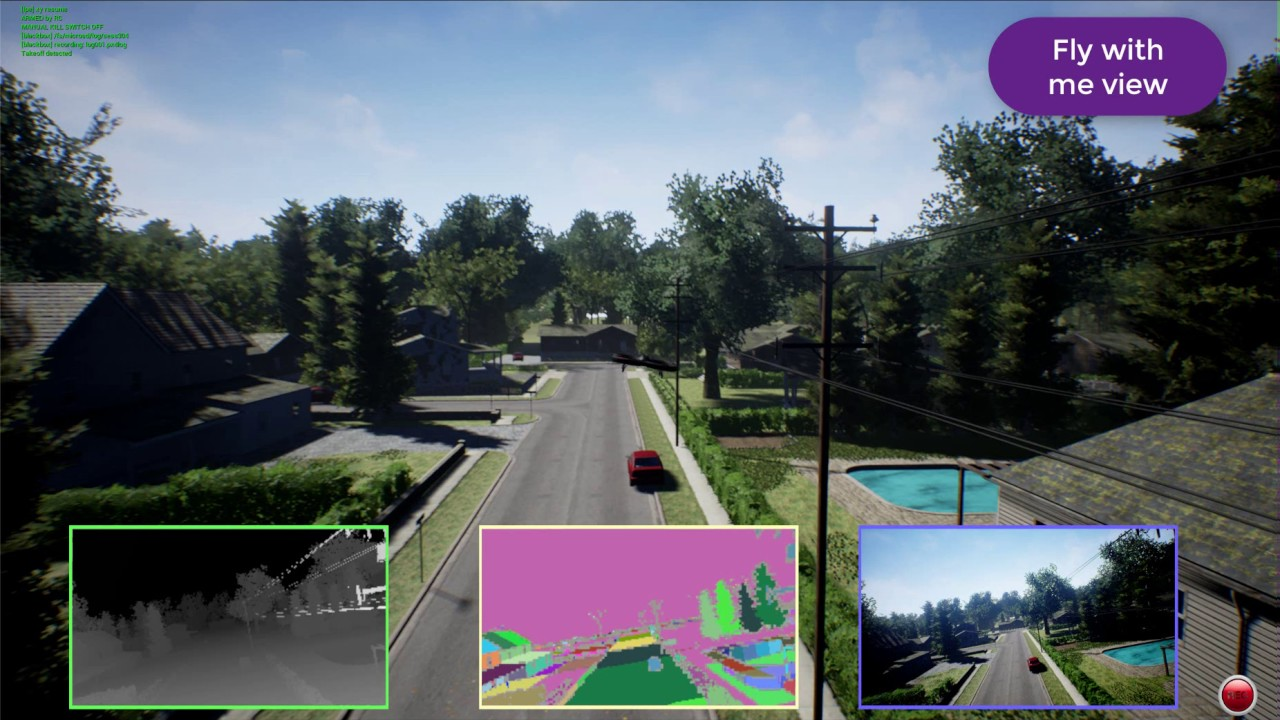
\includegraphics[width=0.49\textwidth]{airsim}
	\caption{SimuladorAirSim.}
	\label{fig-airsim}
\end{figure}

\subsection{Carla SIMULATOR}

Carla és un simulador gràfic realitzat en Unreal Engine; aquest simulador té la finalitat de generar imatges en un entorn simulat amb el màxim realisme per generar imatges que poden utilitzar en xarxes neuronals amb l'objectiu de conduir un cotxe autònom de forma segura, tenint en compte els casos improbables que són difícils de generar en món real. Carla té les funcionalitats següents: simulació de cotxes, vista depth, vista de segmentació, simulació de trànsit, simulació de vianants, control dels actors (trànsit, vianants, càmeres, etc) amb un script python, etc.

\begin{figure}[!h]
\centering
  	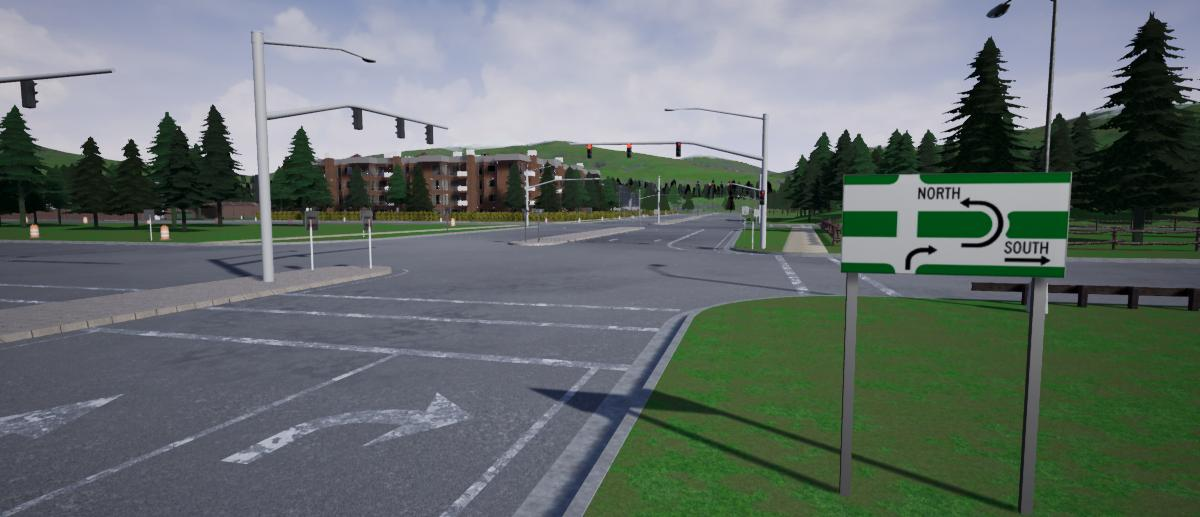
\includegraphics[width=0.49\textwidth]{carlatown}
	\caption{Exemple de Carla.}
	\label{fig-airsim}
\end{figure}

\subsection{LESS}

LESS és un model de la radiació (es pot veure un exemple, en la figura \ref{fig-lessradiacio}) generat en un objecte/terreny tridimensional per a diferents raigs generat a partir tècniques de ray-tracing, d'aquesta forma és capaç d'utilitzar-ho per simular dades i imatges sobre escenes tridimensionals realistes. Aquest model implementa un mètode de seguiment de fotons ponderats per simular l'efecte de la reflectància bidireccional multiespectral.

\begin{figure}[!h]
\centering
  	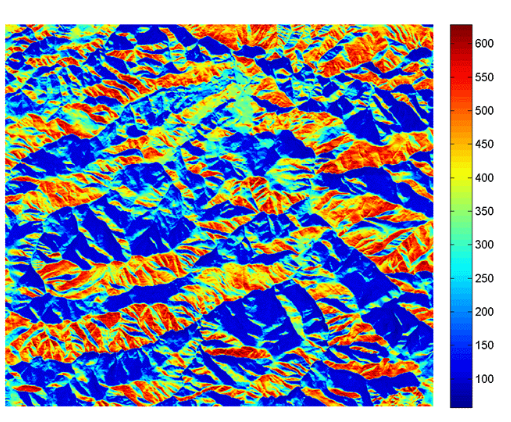
\includegraphics[width=0.4\textwidth]{lessradiacio}
	\caption{Exemple dels resultats de la radació d'un terreny.}
	\label{fig-lessradiacio}
\end{figure}

\subsection{DIRSIG}
El model de Digital Imaging i Remote Sensing Generation Image (DIRSIG) és un model de generació d'imatges sintètiques desenvolupat pel laboratori de Digital Imaging i Teledetecció del Rochester Institute of Technology. El model pot produir imatges d'una banda, multiespectrals o hiperspectrals a partir del canal visible de la regió tèrmica d'infrarojos de l'espectre electromagnètic. Podeu veure un exemple generat per DIRSIG sobre la figura \ref{fig-tacoma}.

\begin{figure}[!h]
\centering
  	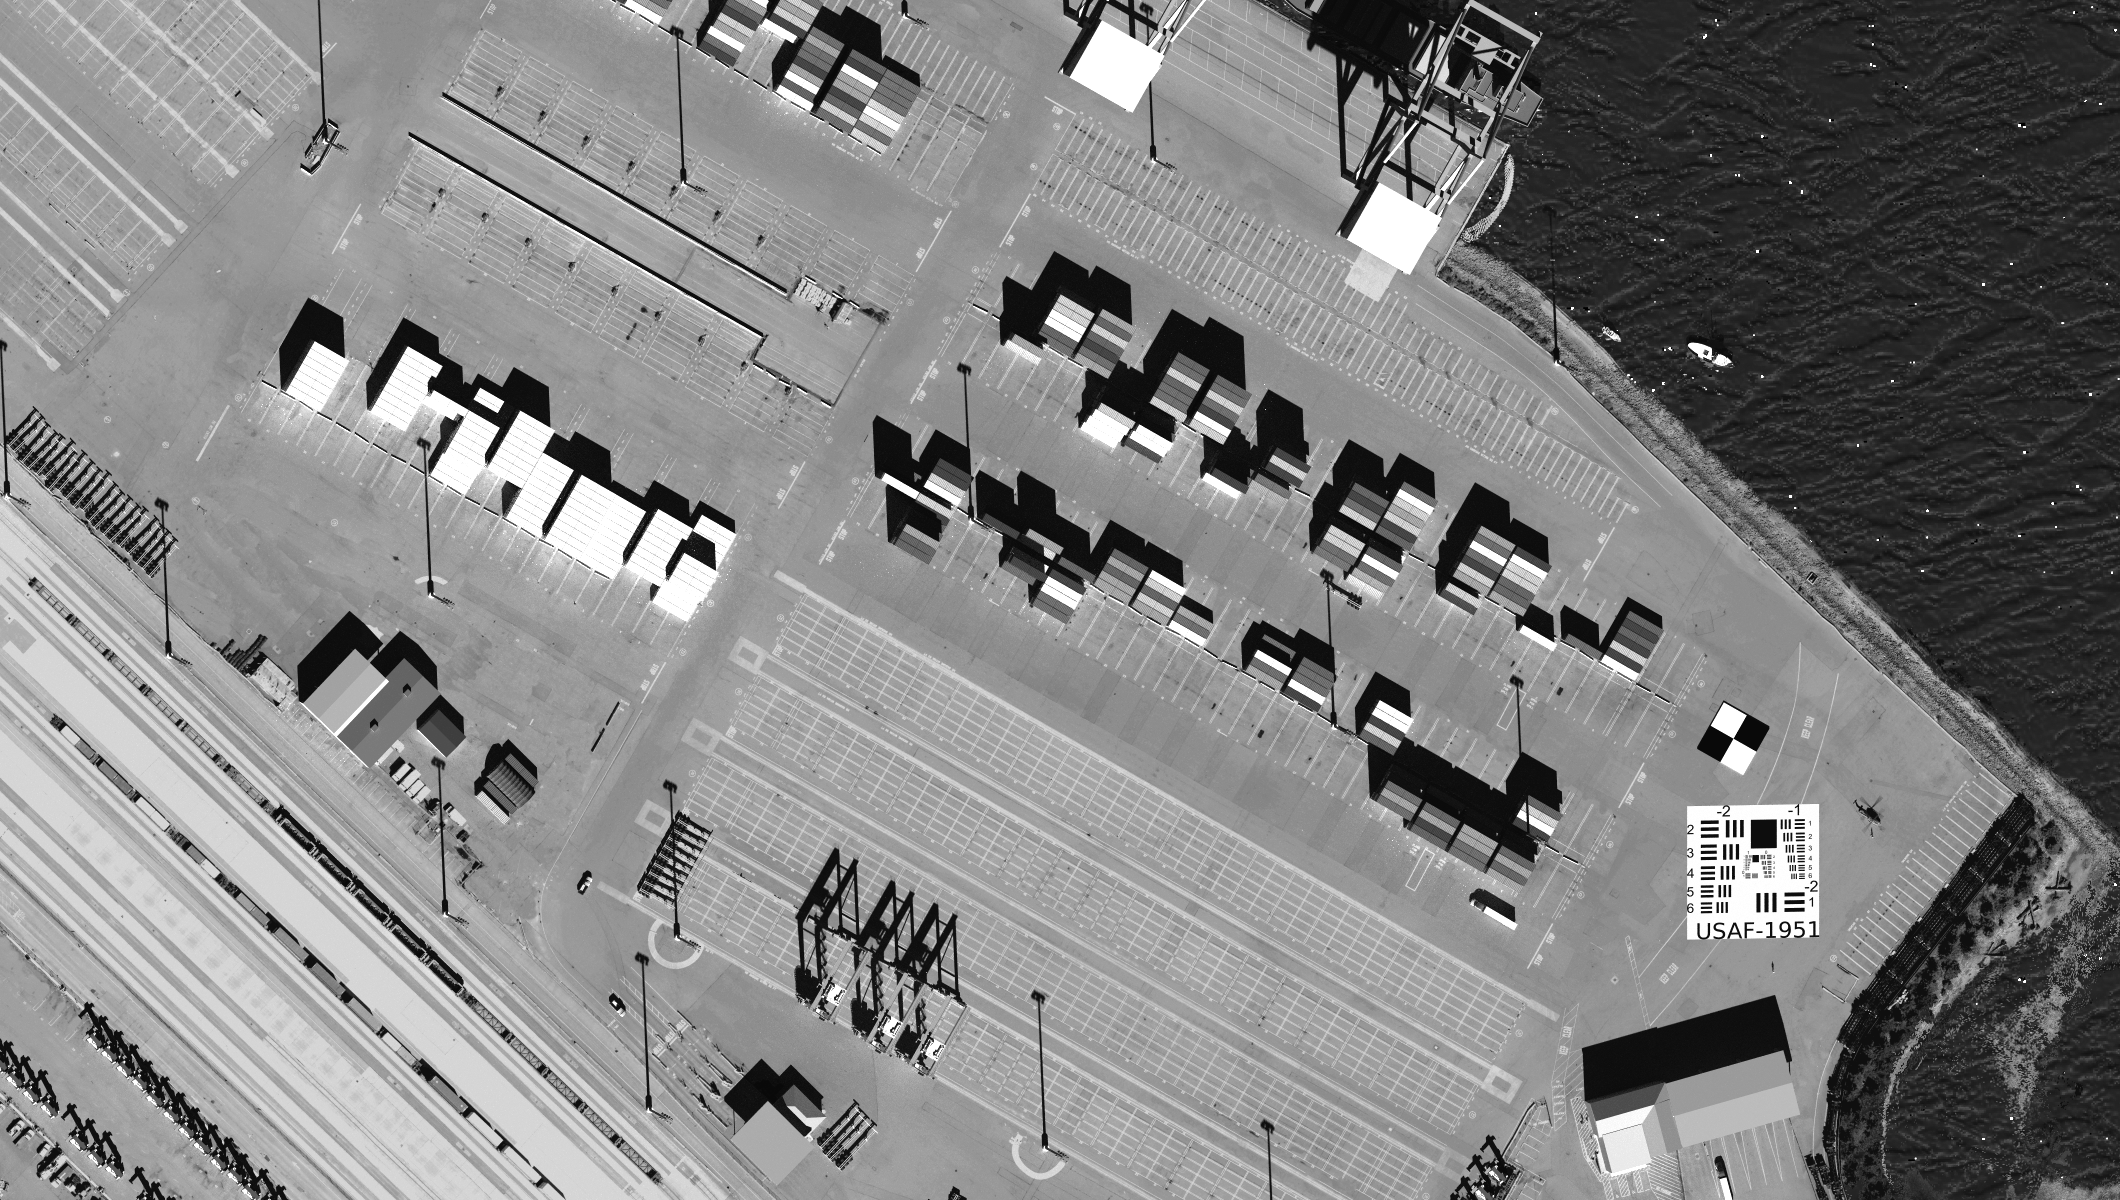
\includegraphics[width=0.49\textwidth]{tacoma}
	\caption{Imatge del port de Tacoma.}
	\label{fig-tacoma}
\end{figure}

\subsection{Google Earth Engine}

Google Earth Engine és un projecte de Google dedicat a oferir les eines necessàries per poder analitzar i visualitzar dades geoespacials destinades a estudis acadèmics, institucions sense ànim de lucre, empreses i governs. Les principals característiques de Google Earth Engine són:

\begin{itemize}
\setlength\itemsep{0em}
  \item Podem treballar amb conjunts de dades de diferents satèl·lits com LANDSAT, MODIS, SENTINEL, etc.
  \item Incorpora un entorn de treball per manipular les dades i una àmplia API que ens permet combinar imatges de diferents espectres, veure-les en un mapa del món, exportar dades a Google Drive, etc.
\end{itemize}

\section{Estructura del projecte}
In order to determine the project structure, it is study the diverse alternatives viewed in section \ref{estatart}. The structure of AirSim and Carla will be analyzed with the objective of deciding the ownership structure and the external libraries to incorporate them into the project.

\subsection{AirSim} 
AirSim is composed of multiple modules written in various languages, as can be seen below:

\begin{itemize}
\setlength\itemsep{0em}
	\item \textbf{AirLib (C++)}: Module for Unreal Engine that provides the base classes to communicate through the RPC protocol and control the simulated vehicles.
	\item \textbf{DroneServer (C++)}: Server to receive orders from RPC client.
  	\item \textbf{DroneShell (C++)}: Shell client to send orders to the Server.
  	\item \textbf{PythonClient (Python)}: Client to send orders trough RPC, also includes code to the manipulation of images.
  	\item \textbf{SGM (C++)}: Code to manipulate images and generate the segmentation view.
    \item \textbf{Unity (C\# i C++)}: Unity version, includes a modules to see the AirSim information.
    \item \textbf{Unreal Engine (C++)}: Unreal version, includes a modules to see the AirSim information.
\end{itemize}

\subsection{Carla SIMULATOR}

Carla SIMULATOR is composed of multiple modules as you can see in the figure \ref{fig-carlamodules} written in multiple languages. The modules of Carla are:

\begin{figure}[!h]
  	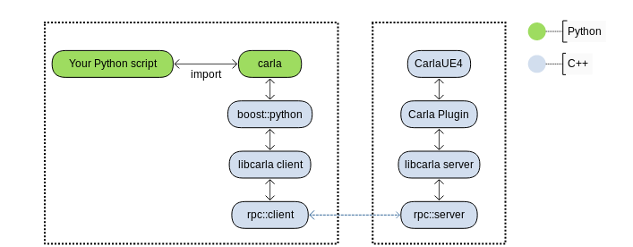
\includegraphics[width=0.52\textwidth]{carlamodules}
	\caption{Relation between the modules of Carla.}
	\label{fig-carlamodules}
\end{figure}

\begin{itemize}
\setlength\itemsep{0em}
 \item \textbf{LibCarla (C++)}: The main library of Carla, is in charge of the logic of the simulation.
 \item \textbf{Unreal (C++)}: Graphic engine with the Carla plug-in, this includes all the functionalities added to Unreal.
 \item \textbf{PythonAPI (Python)}: The API allows sending orders to the Carla module that works like server, this API it is useful to make own scripts.
\end{itemize}


\subsection{The structure chosen}

In this section multiple projects with similar characteristics have been analyzed to decide the structure that can be seen in figure \ref{fig-dronsimulatormodules}, in which some modules from other open source projects will be used. Its make this decision due to the fact that the other projects are based on the creation of terrain predefined on Unreal Editor, the opposite to the finality of this project in which its make terrain automatically provided by real data.

\begin{figure}[!h]
\centering
  	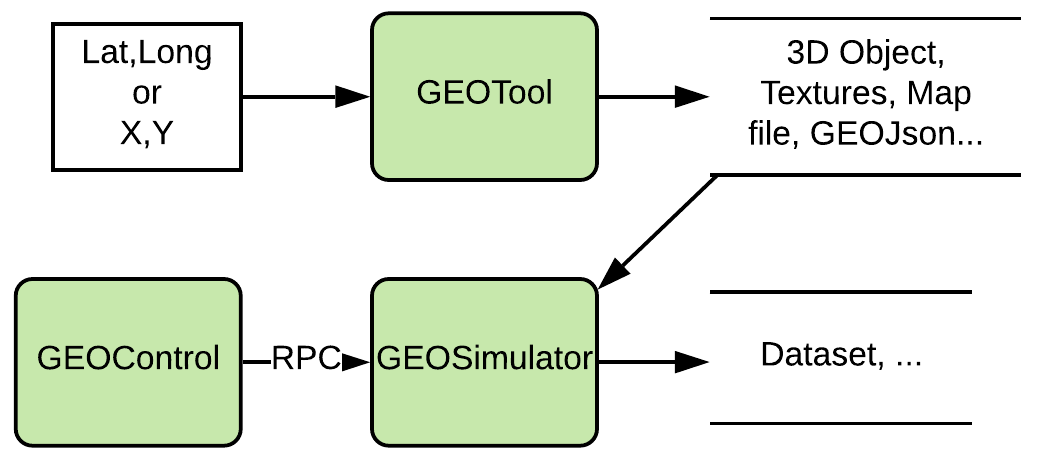
\includegraphics[width=0.45\textwidth]{structuretfg}
	\caption{Structure of GEOSpectralSimulator.}
	\label{fig-dronsimulatormodules}
\end{figure}

The project is consisted of these modules:

\begin{itemize}
\setlength\itemsep{0em}
  \item \textbf{GEOTool (Python)}: This module has the goal of providing the needed tools for obtaining and adapting the data from some standards for geographical data web-service with the objective of can import this data on any graphic motor, it can generate diverse layers of data for the downloaded terrains as textures (RGB, infrared, etc.), geojson, etc. 
  
  \item \textbf{ScriptAPI (Python)}: This module provides the interface to control the simulator trough scripts and trajectories files, allow it to control the vehicle, cameras, generate images for the dataset, etc. Also can implements extra functionality as generation of noise to the vehicle and more.
  
  \item \textbf{Unreal Engine Simulator (C++)}: Based on the Unreal Engine includes the plugins to implement an RPC Server, interface necessary to read files generated by GEOTool and the generation of images.
\end{itemize}

\section{Module GEOTool}

In this section it can seen how the GEOTool module works and what is the functionality implemented, more concretely can see the origin of data, the configuration file, how to prepare data for graphical engines like as Unreal, Unity, OpenGL, etc. Finally the performance of the generation from wavefront object files (.obj) will be analysed.

\subsection{Obtaining data}
\label{getdata}

With the goal of getting geoghrapical data it has been decided that the communication will use standards proposed by Open Geospatial Consortium \cite{ogc}: Web Map Service \cite{wms} in charge of making image data available we take an orthophoto from a geographical region selected and Web Coverage Service \cite{wms} and we get data concerning the elevation of terrains in a concrete geographical region. In order to get that data HTTP requests are made to the web services offered by multiple institutions that follows the standards chosen, and we'll make tests with the Institut Cartogràfic I Geològic de Catalunya \cite{icgc}.

\subsubsection{Configuration file}
\label{section:configfilegeotool}
For determining which data will wish be obtained and where webservices the app accept by command line parameter a file with the configuration in JSON format. This allows determining the properties of the data they want to request as I can see on the appendix \ref{appendix:geotoolconfig}. On this file can configure the next parameters:

\begin{itemize}
\setlength\itemsep{0em}
  \item \textbf{Type}: It refers to the type of coordinates that we will pass, can be latlong or x-y, in the first case it will make the corresponding transformation to the UTM format (x-y).
  
  \item \textbf{Coordinates}: Coordinates on which we want to make the request in the format indicated in the type field. If ``xy'' is selected, the attributes x,y will be defined, and in case of choosing ``latlong" we will define the lat, long attributes.

  \item \textbf{Dimensions}: The dimension field can choose the dimensions that you want to request in pixels, it is composed by:
  
  \begin{itemize}
  \setlength\itemsep{0em}
  \vspace{-0.2cm}
    \item Bbox: Bbox is the dimensions in pixels of geographical area, this is used by all requests to identify the area in a unique way.
    \item Texture: Texture is a resolution in pixels request to the texture image.
  \end{itemize}
  
  \item \textbf{chunks}: The fragments that want to be downloaded, the application calculates the displacement and generates n pieces of width$\times$height.
  \vspace{-0.2cm}
  \begin{itemize}
  \setlength\itemsep{0em}
    \item width.
    \item height.
  \end{itemize}

  \item \textbf{cellsize}: Size of each pixel in meters.
  \item \textbf{meshStep}: The number indicates the quantity of points that wish to skip on the mesh (Default: 1). More information on the section \ref{qualitat}.
  \item \textbf{Wcsurl}: The URL to the web service that will give us the height data.
  \item \textbf{Outputwcs}: Base name of the output files.
  \item \textbf{Formatwcs}: Format of file generated by heightmaps. Available: {\tt raw, obj} (Object 3D).

  \item \textbf{Wmsrequests}: Array with each request that will be for obtaining textures, each item are composed by:
  
  \begin{itemize}
  \setlength\itemsep{0em}
    \item Url: URL to the webservice WMS.
    \item Layers: The layers we want to get from these webservice.
    \item Name: The name of texture, used by the generated files.
    \item Format: Output format. Available: {\tt jpg}.
  \end{itemize}
  
\end{itemize}

\subsection{Generation of terrains from a elevations maps}

This section explains the different ways to generate terrain data that can be interpreted by multiple graphical engines. More specifically, this section shows the raw format and wavefront object.

\subsubsection{Format RAW}

The RAW format is a format based on values of 16 bits, where the value of sea level is 128. All the heights are saved in binary format and put in a file. This format is accepted by the Unreal and Unity land builder, but has dimension limitations; You must meet several specified conditions in the Unreal Editor, this causes you to lose control of the generated mesh, the texture coordinates do not match and the texture that is applied to the mesh will have to adapt. Motivation by which is decide to add the generation of 3d objects in the standard format, generating own objects as you can see in section \ref{mesh3d}.

\subsubsection{Generation of mesh 3D}
\label{mesh3d}
To import land in the graphics engine, it decides to generate a 3D mesh in {\tt obj} format compatible with any 3D editor, graphics engine, etc. This device gives the freedom to control the distance between the vertex, where the texture is applied and which is the normal vector of each vertex to correctly apply the algorithms of illumination.
\\
\\
As the treatment with loops is slow, all the operations are made with the library NumPy take advantage of efficiency incorporates this library with the calculus of matrices. The problem has been adapted to operations of matricial type, you can see the code in the appendix \ref{appendix:generateobj}.
\\
\\
For the generation of objects four types of objects must be defined:

\begin{itemize}
\setlength\itemsep{0em}
  \item \textbf{Vertex}: Are each point in the world. Vertex are referenced in the index according to the elevation grid (1, 2, 3,..., H$\times$W). Each point is multiplied by a K (K represents the distance between two vertex according to the distance that indicate the elevation map obtained).

  \item {
    \textbf{Vertex of texture}: Vertex with two components x and y compressed between 0 and 1 that indicates the correspondence between the points of the texture and location in the mesh. This property is calculated with the equations \ref{equation:u} and \ref{equation:v}.
    \begin{equation}
    \label{equation:u}
    u = f(column) = column / (width - 1)
    \end{equation}
    \begin{equation}
    \label{equation:v}
    v = f(row) = 1 - (row / (height - 1))
    \end{equation}
  }

\vspace{-0.5cm}
  \item \textbf{Normal of vertex}: Vectors indicate the direction in which the light is reflected for each vertex of the object. In order to calculate these normals is necessary, calculate the normal for each face, though these are not included in the final file because the engines generate it by default.

  \begin{itemize}
  \setlength\itemsep{0em}
    \item {
      Generation of normal faces: In order to generate the normals of a face once you know the relation between the faces, we follow the pattern you can see in the figure \ref{fig-normalpattern} where we follow the equation \ref{equation:u} for the calculation of the normal face $\vec{A}$, it makes cross product $\vec{C} = \vec{B}\times\vec{A}$ and finally is normalize the vector $\vec{Normal} = \frac{\vec{C}}{\mid\vec{C}\mid}$.
    }

    \item {
    Generation of the normal for the vertex: In order to generate the vector normal for each vertex, we use the structure that can see in figure \ref{fig-normalpattern} applying the next equation for each vertex where V correspond to the vertices and F corresponds to the faces on the figure \ref{fig-normalpattern}:
      \begin{equation}
      \vec{NormalV} = \vec{F_1} + \vec{F_2} + \vec{F_3} + \vec{F_4} + \vec{F_5} + \vec{F_6}
      \end{equation}
      \begin{equation}
      \vec{NormalV} = \frac{\vec{NormalV}}{\mid\vec{NormalV}\mid}
      \end{equation}
    }
  \end{itemize}

  \item \textbf{Faces}: In this step it is determined which is the union of vertices that will be used to generate the different faces of the mesh, in this implementation it is decided to make a triangulation, in other words, that is for each square of the own mesh two triangular faces will be generated. It is important generate the faces in correct order, writing the vertices following an opposite clockwise order, in this way the graphic engine determines that the normal face will point up by displaying the 3D mesh correctly.
\end{itemize}

\begin{figure}[!h]
\centering
  	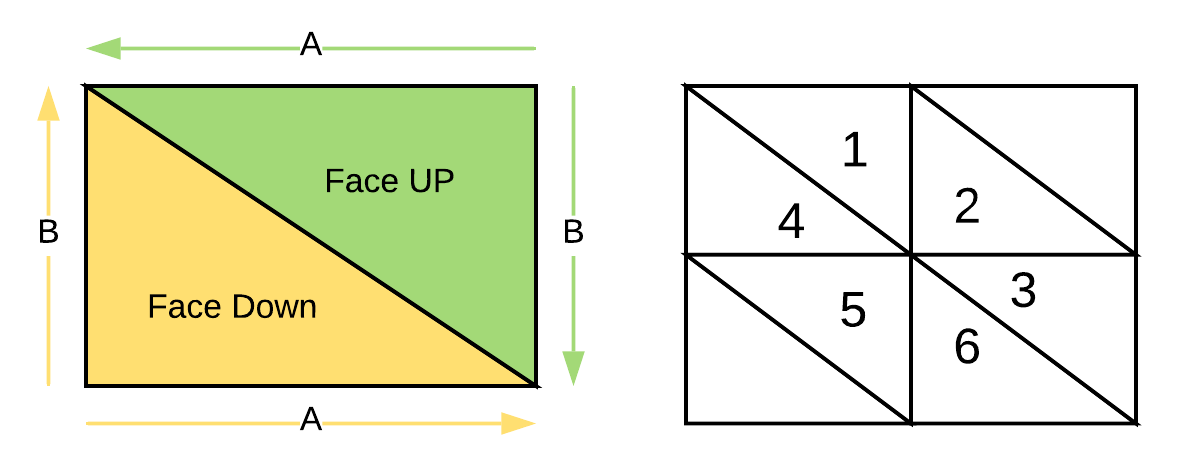
\includegraphics[width=0.49\textwidth]{patternmeshgeneration}
	\caption{Pattern for the calculation of normal on the faces (Left) and vertex (Right).}
	\label{fig-normalpattern}
\end{figure}

Once the generation process has been completed, the application will generate a mesh that can be opened in any editor. As it can be seen in the figure \ref{fig-meshlab} where it is open using the MeshLabs software.

\begin{figure}[!h]
\centering
  	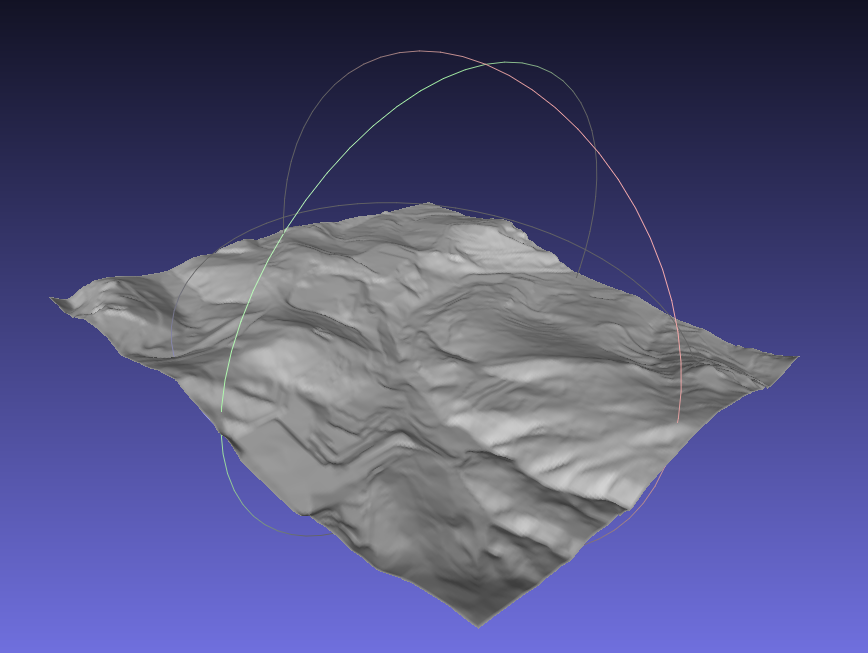
\includegraphics[width=0.49\textwidth]{mesh_example_meshlab}
	\caption{Terrain mesh visualized in software MeshLab.}
	\label{fig-meshlab}
\end{figure}

\subsubsection{GEOJson associated at the terrain}

In order to localize the terrain generated in other software that's working with geospatial data or in within the Unreal simulator itself, a GEOJson file it is included. This file indicates which belongs to the files generated. An example of this can be seen in the appendix \ref{appendix:geojson}.

\subsection{Time of generation}
In this section the two versions implemented are analyzed to see the difference in generation time. This is an important point for future implementations in which the goal might be to implement a viewer in real time, where new data loads as the user moves on the world.
\\
On the figure \ref{fig-meshtime} the differences in time between the version using for loops and the version using the NumPy library can be seen. The implementation using the library NumPy is 24 times faster for a size of 500$\times$500, this is due to the fact that NumPy is optimized for parallel processing of vectorial data.

\begin{figure}[!h]
\centering
  	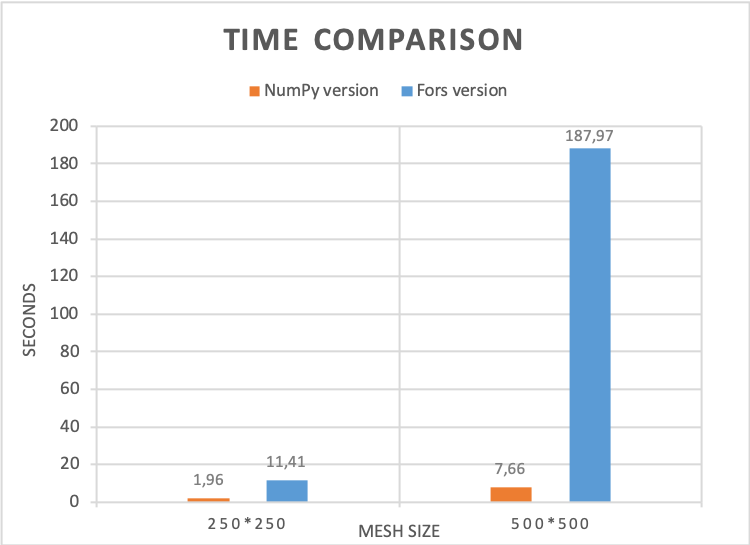
\includegraphics[width=0.4\textwidth]{meshtime}
	\caption{Graph with the time of generation of a mesh according to size.}
	\label{fig-meshtime}
\end{figure}

\subsection{Quality}
\label{qualitat}
This section shows the results of reducing the quality of the terrain, both qualitatively (visual difference) and quantitatively (size in bytes). In order to make this reduction skips of size "meshStep" are made, set in the JSON configuration file. Test with powers of 2 (2, 4, 8, 16,...) are made on the matrix of points itself, using the terrain of size 300$\times$300 pixels.
\\
\\
As it can be seen in the figure \ref{fig-qualitatmegas} when reducing the amount of points, the size on the disk is exponentially reduced, making the file load faster on the Unreal environment. As it can be seen in the figure \ref{fig-qualityvisual}  the loss of quality is visible, taking as a reference the mountain in the background it can be seen the loss of definition at the top of the mountain. It can be considered that visually, when "meshStep" is configured as 1 or 2, the loss of quality is not noticeable. At 4, it can be noticed slightly, and finally at levels 8 and 16 a noticeable loss in quality is noticed. This can be seen in the peak of the mountain, which has been simplified, as opposed to when it is configured with a value of 1, where it shows the mountain with more definition.

\begin{figure}[!h]
\centering
  	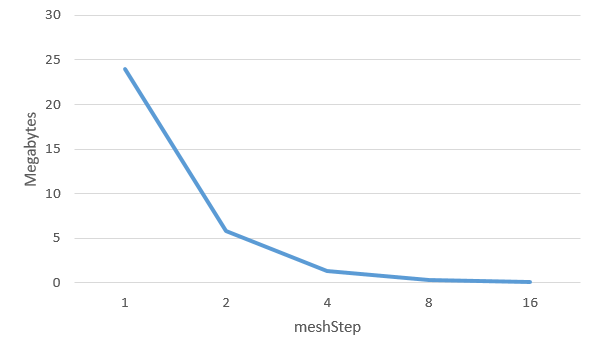
\includegraphics[width=0.4\textwidth]{qualitatmegas}
	\caption{Graphic with the size occupied on hard disk varying the ''meshStep'' parameter for a terrain of size 300$\times$300.}
	\label{fig-qualitatmegas}
\end{figure}

%TODO Cambiar grafico para que se vea más el cambio.
\begin{figure}[!h]
\centering
  	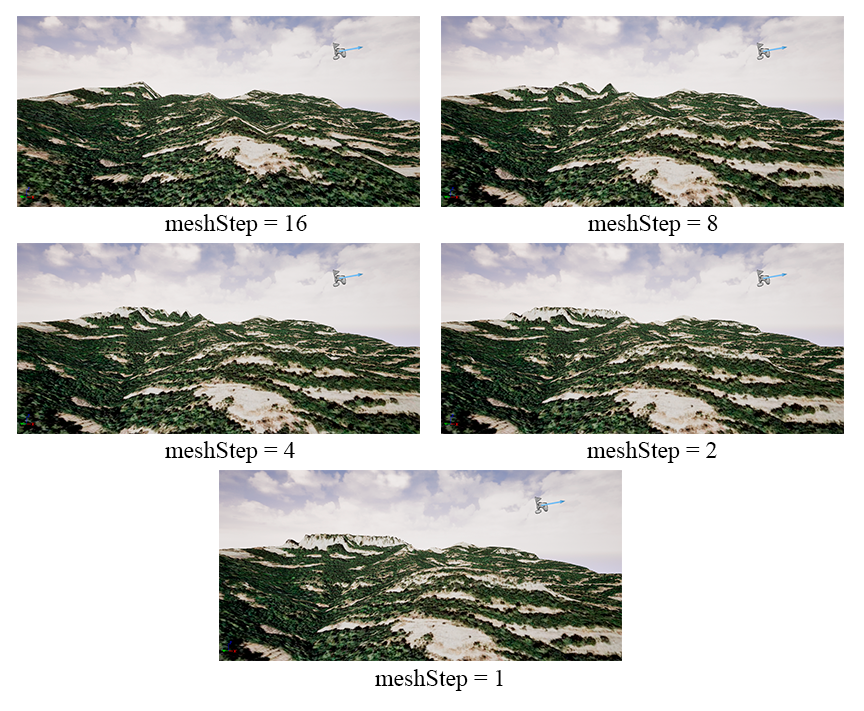
\includegraphics[width=0.5\textwidth]{quality/quality}
	\caption{Visual comparison of the effects produced by the level quality.}
	\label{fig-qualityvisual}
\end{figure}

\subsection{Map file}
 
A file which will be read later on the simulator is generated.  The map's file is divided in a set of smaller parts, downloaded in a request done through GEOTool. These parts contain basic information: location in the real world, size, size of each pixel, textures we want to load, etc. The file can be modified manually to modify locations, add textures that have not been acquired through GEOTool (it's necessary that the portions of terrain have a texture configured with the same name, otherwise it won't load), etc. An example can be seen in the appendix \ref{appendix:mapjson} .

\section{Module: Simulator}

In this section the multiple parts of which the module of simulation it is composed are explained. The objective of this module is to make an available a tool that allows to simulate a travel with a generic vehicle above a terrain, getting images from multiple cameras on board of the vehicle. A way to make this is providing the interface control of the vehicle with an external script sending commands with the RPC Protocol, in this case, it is implemented on the server as it can be seen in section \ref{rpcserver} and controllled with a client implemented in a module as it can be seen in the section \ref{modulescript}.

\subsection{Visualization and control of the vehicle}

The goal of this part is to provide the interface for moving a generic vehicle in the simulated world, this vehicle is configured with several cameras that are displayed on the screen and that can generate images of what they see. Using this, the possibility of viewing the same area in multiple perspectives is added. As an example, you can see the zenith view in the figure \ref{fig-montserratir}.

\begin{figure}[!h]
\centering
  	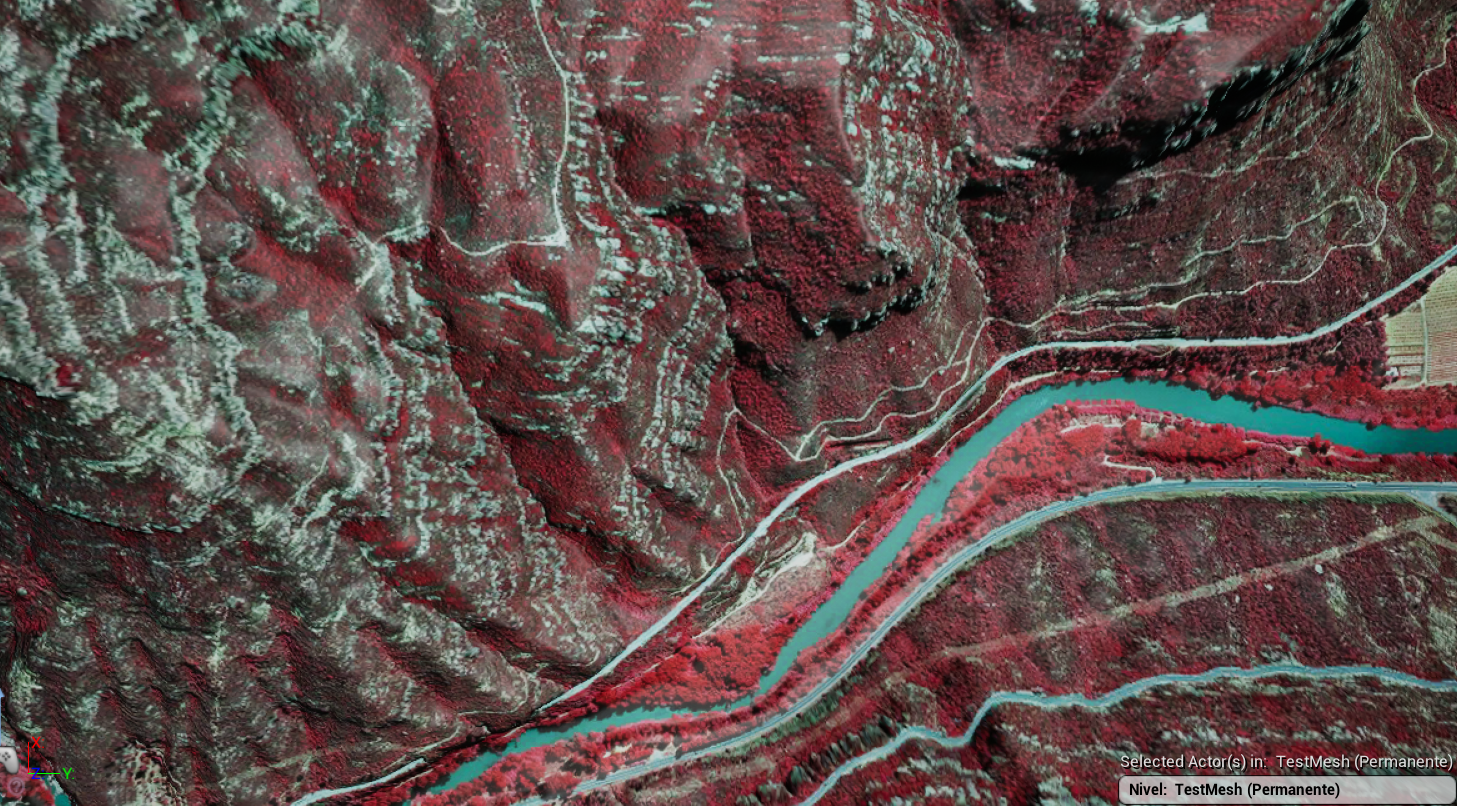
\includegraphics[width=0.49\textwidth]{cenitalviewir}
	\caption{Infrared view of Montserrat in zenith position.}
	\label{fig-montserratir}
\end{figure}

\subsubsection{Remote control}
\label{rpcserver}

In order to control the vehicle remotely, a communication using the RPC protocol (Remote Procedure Call) it is implemented, more specifically, it is using the Rpclib \cite{rpclib} library for C++. This server is implemented on the Unreal module, the RPC server management is done through a class (AVehiclePawn) that can be inherited so that it basically offers the interface necessary to control a vehicle. The following actions are implemented: initialize/stop the RPC server, change the position of the vehicle, change rotation of the vehicle or cameras (Implemented with LookAt), ask for images from one of the cameras to be generated, etc.
\\
The assignment of the functionalities is done in the function {\tt void BindFunctions(rpc::server* server)} which receives the instance of the server, this function can be overridden to later be added to legacy classes with more functionality as it can be seen in the appendix \ref{appendix:extendrpc}. By default the AVehiclePawn class allows us to call the following RPC functions:

\begin{itemize}
\setlength\itemsep{0em}
\item {\tt setLocation(double x, double y, double z)}: Send the location on which one place the vehicle.

\item {\tt setLookAt(double x, double y, double z)}: Send a vector with the position in the world you want to look at, so that at which point the simulator should keep the camera's eyes.

\item {\tt setLocationAndLookAt(double x, double y, double z, double lx, double ly, double lz)}: The function that implements the two previous calls in a single call.

\item {\tt setCameraLookAt(int cameraId, double x, double y, double z)}: A function that choose a camera and configure in what direction the camera look at.

\item {\tt getImage(int idCamera, std::string path, std::string channel)}: Generates images using the following information: the camera that will generate the image, the place where to save the image and the texture from which you want to obtain the image. All this is done synchronously, to guarantee that the image is generated in the correct position.
\end{itemize}

\subsubsection{Sky visualization}

\begin{figure*}[!h]
\centering
  	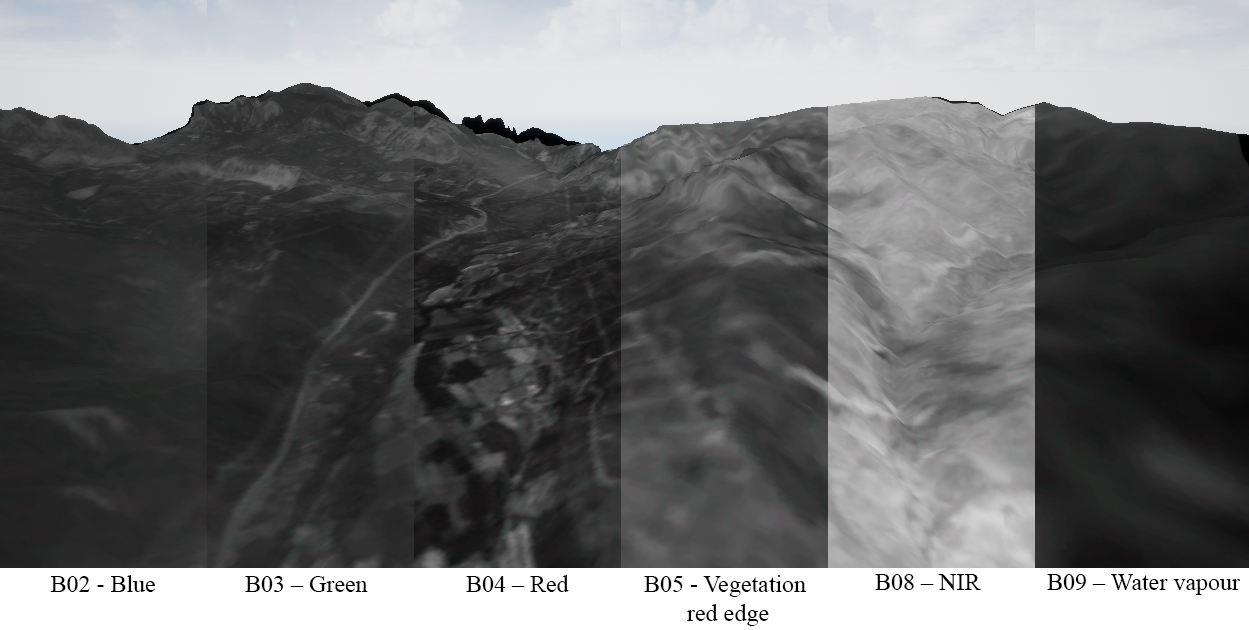
\includegraphics[width=1\textwidth]{multispectral/bands}
	\caption{View of ''Sales de Pallars'' in six spectral bands differents.}
	\label{fig-bands}
\end{figure*}

In order to implement the sky, the native module of Unreal is used, where a sphere is generated on which the sky is rendered. This sky has multiple parameters for configuring the sky in multiple ways, some of the things that can be done are: determining the sun position, the lighting of stars, the quantity of clouds, the velocity of the clouds, etc.
\\\\
This allows to generate synthetic images in different moments of the day with a different lighting, to generate more complex datasets. On the other hand, it is applied without shadows because the shadows are generated by Unreal, if these shadows are generated by the 2 bands, they overlap generating an undesirable strange effect. An example of differents hours of the day can be seen in figure \ref{fig-sky}.

\begin{figure}[!h]
\centering
  	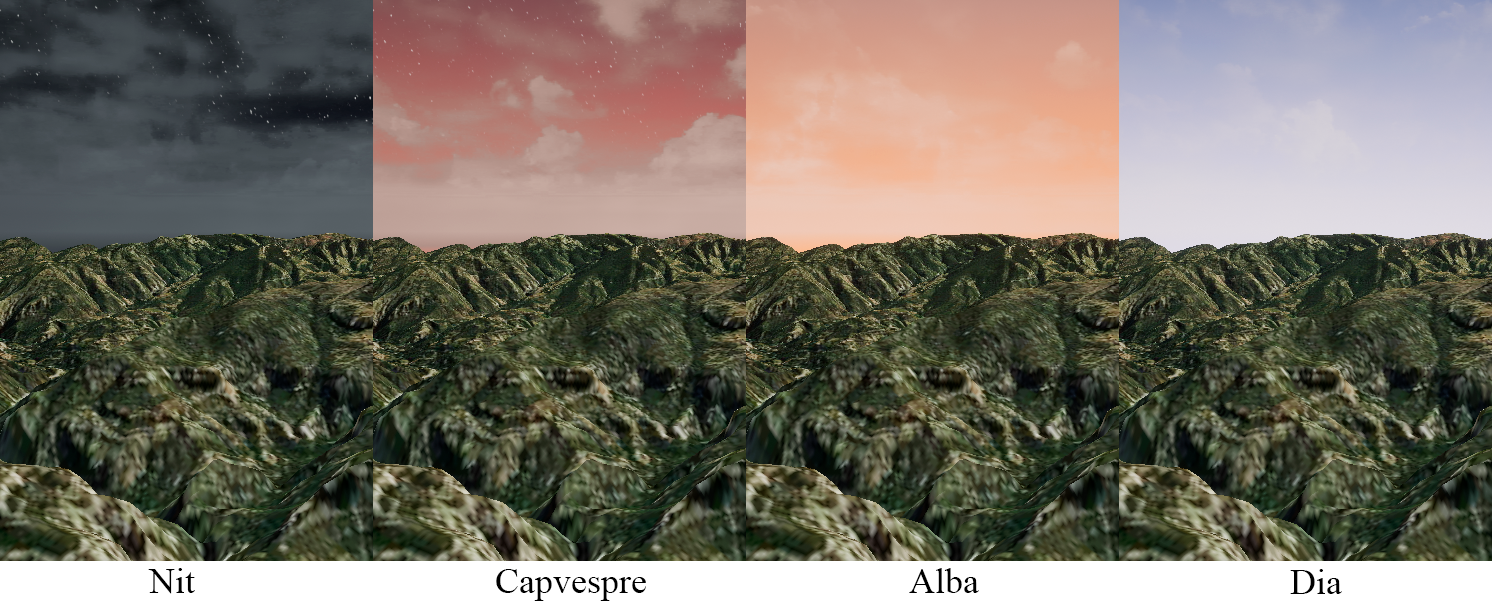
\includegraphics[width=0.49\textwidth]{sky/sky}
	\caption{Example of differents sky.}
	\label{fig-sky}
\end{figure}

\subsection{Terrain}
The terrain is loaded through code executed at runtime obtaining the obj file and this file is processed to generate a UProceduralMesh \cite{uprocedural} that contains the mesh generated with the api of this class to generate meshes in runtime. To generate this mesh it must be considered that Unreal works with a different system of coordinates, it is inverted respective to the UTM model on the y axis. Due to this, it is necessary to make the necessary changes.
\\
\\
This mesh is loaded on the world and it is represented by the class ``MapChunk'', to which a dynamic material that contains the loaded textures for generate the different visualizations is assigned. The texture can be any image prepared to use as a texture on Unreal, giving the possibility of seeing RGB, infrared, multispectral bands, indexes generated by the multispectral data, etc.

\begin{figure*}[!h]
\centering
  	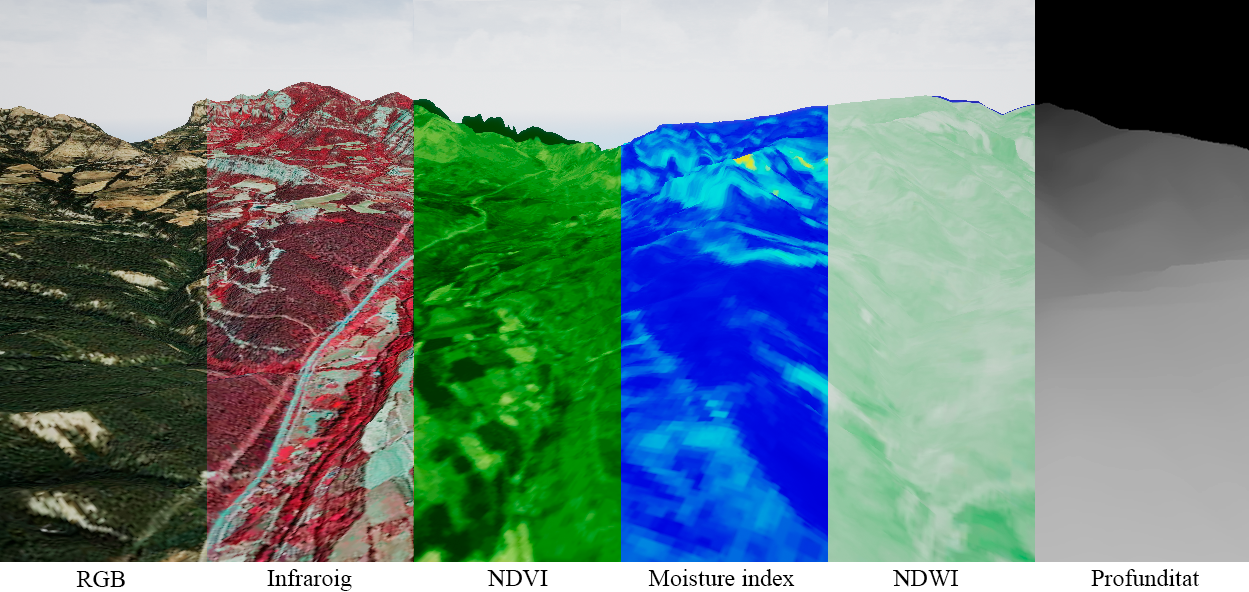
\includegraphics[width=1\textwidth]{multispectral/spectralindexes}
	\caption{View of ''Sales de Pallars'' in RGB, infrared, NDVI, moisture, NDWI and depth.}
	\label{fig-spectralindexes}
\end{figure*}

\subsection{Results of visualization of terrains}
In this section can see the results obtained from the 3D terrains generated by the module GEOTool and apply multiple visualizations from origins as textures or shaders obtained from different sources. More specifically, the RGB and infrared views are obtained from ''Institut Cartogràfic de Catalunya'', the multispectral data is obtained from the browser EO Browser \cite{eobrowser} and the depth data is generated applying a shader to the scene.
\\
\\
You can see in Figure \ref{fig-bands} how it has been applied to a terrain that corresponds to "Sales de Pallars", different multispectral bands obtained from the satellite Sentinel 2 \cite{sentinel2}. The first three bands B02, B03 and B04 correspond to the bands of colours, the band B05 corresponds to the fast change of the reluctance that is produced in the vegetation in a range near of infrared, the band B08 obtains NIR \cite{nir} data and the B09 is able to detect water vapours.

With these bands composed data from multiple spectrums that can be applied to multiple scopes is obtained. In figure \ref{fig-spectralindexes} some examples can be seen, between them the indexes are:

\begin{itemize}
\setlength\itemsep{0em}
\item 
{
	NVDI \cite{ndvi}: Based on the combination of the bands (B08 - B04)/(B08 + B04), index used to see the farming state.
}
\item
{
	Moisture index \cite{moisture}: Based on the combination of the bands (B8A - B11)/(B8A + B11), indicates the proportion of precipitation that is needed so that satisfy the needs of vegetation.
}
\item
{
	NDWI \cite{ndwi}: Based on the combination of the bands (B03 - B08)/(B03 + B08), the index is used to determine the hydrique stress of the vegetation, saturation of the humidity in the land or limit the mass of water a lakes or reservoirs.
}
\end{itemize} 

The last view of the figure \ref{fig-spectralindexes} the depth or proximity can be seen using  algorithms of 3D reconstruction with monocular stereo, prevention of collisions, algorithm of multiview stereo, etc.

\subsection{How to interact with the simulator}
In order to interact with the simulator the following keys have been defined:

\begin{itemize}
\setlength\itemsep{0em}
\item A,W,S,D: Left, Front, Back, Right movement of the vehicle.
\item Alt, SpaceBar: Down and up the vehicle.
\item Q,E: Left and right rotation of vehicle.
\item Y: Starts an RPC Server
\item U: Stops an RPC Server.
\item H: Show/Hide the visualization of vehicle.
\item K: Save image in the simulator folder from the second camera.
\end{itemize}

\section{Scripting module}
\label{modulescript}

This section contains the explanation of the main points of the scripting module with which the simulator is controlled, in a way that allos to reproduce travels, read trajectories from files, generate images, generate noise to the trajectories, etc.

\subsection{Paths}
The scripting module allows to make travels, read trajectories created in a real world (adapt this to the right format) or generate synthetic this way can recreate on the simulator a trajectory done previously were able reproduce so many times, this allows to do multiple tests with different visualizations of the terrain. For this finally its generate a file that explained in the section \ref{file-trajectories}.

\subsubsection{File of paths}
\label{file-trajectories}
This section explains how to form the path file and the file to place the cameras. The file is in CSV format and can be read from the GEOControl module to tell the simulator the positions of the vehicle and where both the vehicle and the cameras should look, in coordinates of the world.

The file controls the vehicle is composed by the next fields:

\begin{itemize}
\setlength\itemsep{0em}
\item Time: Time in milliseconds from start of the script.
\item x, y, z: Position X, Y, Z in UTM format.
\item LookX, LookY, LookZ: Position X, Y, Z to which we look in UTM format.
\end{itemize}

The file controls the cameras are in another file composed of the fields:

\begin{itemize}
\setlength\itemsep{0em}
\item Time: Time in milliseconds from start of the script.
\item cameraId: The Id of the camera that want to modify.
\item LookX, LookY, LookZ: Position X, Y, Z to which we look in UTM format.
\item GetImage: Boolean (0 or 1) that indicates if you want to generate an image from this camera in this instant of time.
\item Channel: Textures of which we want to obtain images separated by \textbar.
\end{itemize}

An example from the CSV file generated with Excel can be seen in the appendix \ref{appendix:fitxerscsv}.

\subsection{Noise simulation}

Vehicles experience sudden movements due to wind, asphalt conditions and other factors. To simulate this, noise has been introduced in the trajectory of the tests. During the firsts tests, noise was generated through code, but that way the tests can't be reproduced multiple times, that strategy was dismissed. After that, the noise was introduced directly in the CSV files pertaining to the trajectory. This option is better because it allows to work with external files produced by real vehicles and drones, which guarantees that the tests can be reproduced multiple times.

\subsection{Generation of Datasets}
One of the objectives of this project is giving the possibility of generating datasets of synthetic images satellite data, in order to be able generate datasets the field ``GetImage'' is used, as seen in section \ref{file-trajectories}, which generates an image every time it finds this field.

In the figure \ref{fig-dataset} there is a little example with a few images of a tour on which the camera its fixed with a concrete point that it is left behind with the passage of time.

\begin{figure}[!h]
\centering
  	\includegraphics[width=0.49\textwidth]{dataset/dataset}
	\caption{Set of images generated by GEOControl.}
	\label{fig-dataset}
\end{figure}

\section{Full workflow to generate a dataset}

This sections shows an example of the workflow that can be achieved with the modules generated on this project. This will show how to use them and some examples of new applications that can be developed using this project as a base.
\\
\\
First, the GeoTool module is used to obtain data, with the goal of obtaining the coordinates of the area which we want to obtain. For this, we can use apps like Google Maps, which is used in this case to download the zone of ``Volcan de Santa Margarita''. Approximate coordinates are chosen (lat 42.130596, long 2.521956) to obtain the sorrounding area. Once chosen, the JSON that can be seen in section \ref{section:configfilegeotool} is configured. Once the process is completed, the module is called with the following command : {\tt ./GEOTool.sh config.json} (The requirements to run this application can be seen in the appendix \ref{appendix:requirementsgeotool}). Once the process is over, it generates a series of files, as it can be seen in figure \ref{fig-filesgeotool}.

\begin{figure}[!h]
\centering
  	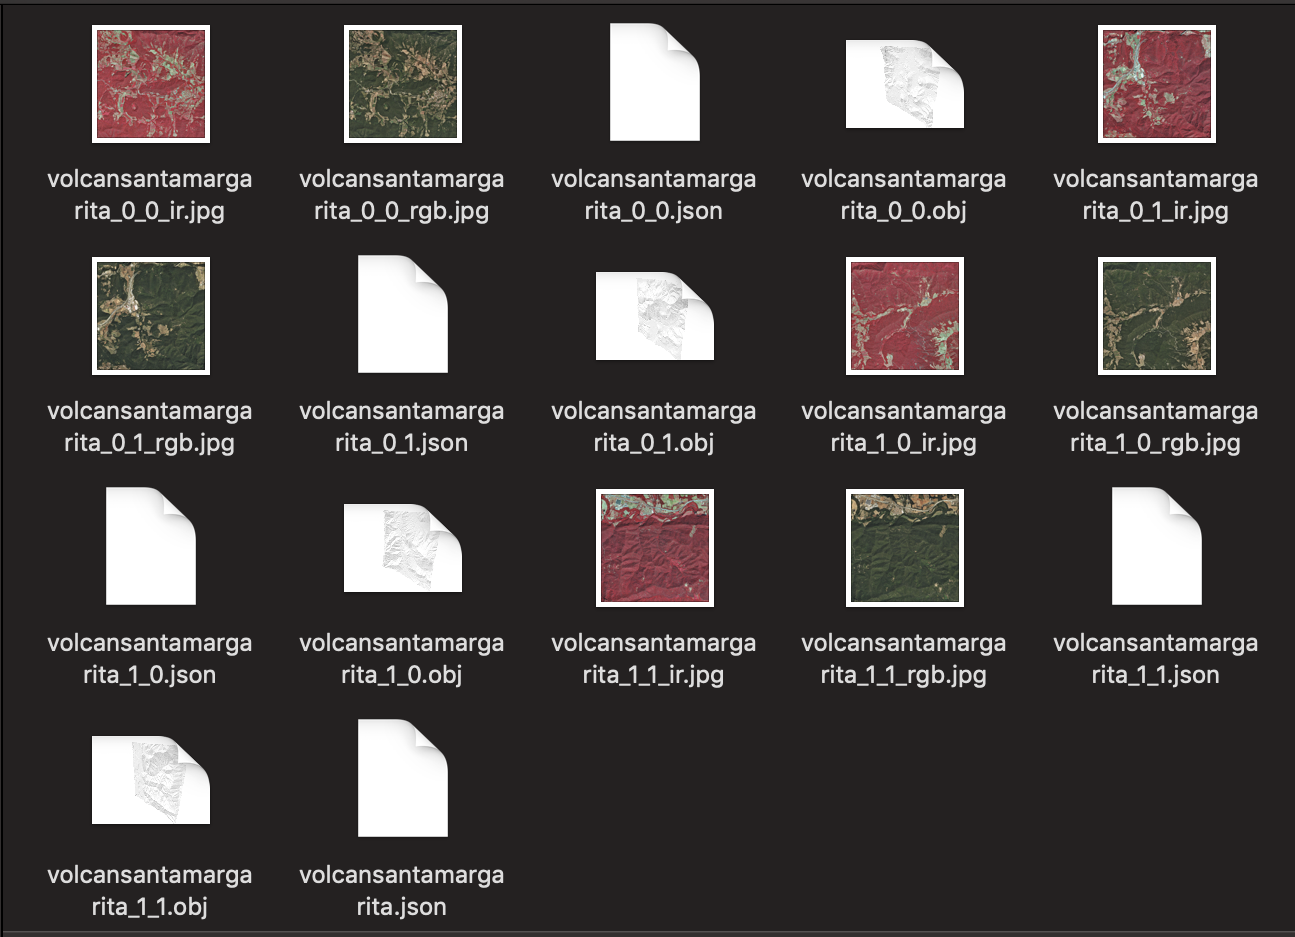
\includegraphics[width=0.49\textwidth]{filesgeotool}
	\caption{Files generated by GEOTool.}
	\label{fig-filesgeotool}
\end{figure}

Once the map is generated, the files will be added to the ``Maps" folder that's next to the executable generated by Unreal, and the simulator will be run with the following command {\tt ./GEOSimulator.sh -folderMap=''Maps/volcan/'' -map=''volcan.json''} (The requirements to run this application can be seen in the appendix \ref{appendix:requirementsgeocontrol}). Once the simulator has initialized, the interface can be seen in the upper left corner, which shows the position in the world where the vehicle is located and the state of the RCP server. An example can be seen in figure \ref{fig-workflowsimulator}.

The RPC server can be initialized with the Y key, and once this is done, the module that controls the vehicle and requests the generation of images will be invoked.

\begin{figure}[!h]
\centering
  	\includegraphics[width=0.49\textwidth]{simulatorworkflow}
	\caption{Simulator view.}
	\label{fig-workflowsimulator}
\end{figure}

With the files containing the trajectories already created as indicated in section \ref{file-trajectories}, the GEOControl module can be invoked with the following command {\tt ./GEOControl.sh filevehicle.csv filecamera.csv}, which executes and generates the dataset in the outputs folder. An example can be seen in figure \ref{fig-dataset}.

\section{Conclusions}

This project shows how to obtain textures and elevation maps originated from satelites. This information can be manipulated to generate indexes, new information generated through neural networks, etc. The treated data is transformed into 3D information that can be interpreted by graphical engines line Unreal Engine. Aspects like the time needed to generate the 3D model are used to see the effect of libraries like NumPy during the manipulation of matrixes, accelerating the process thanks to parallelism. The effect can be seen both in the faster times and in the quality of the meshes with the reduction of the number of points used to generate the 3D model used to render models of big sizes.

The section pertaining to the simulation module shows the information in a 3D enviroment generated with Unreal Engine. We can add cameras to a simulated vehicle and see different perspectives of the same information. To do this, another module has been created, which sends commands to a RPC server implemented in Unreal Engine, in which we can move, choose where the vehicle looks in the real world, where cameras point to and obtain the images captured by the cameras.
The tests, which were performed with data from Satelites like the Sentinel 2, show how this information is represented in the simulated enviroment, which use has each type of data and what possibilities the simulator offers when seeing this information.

The section pertainten to the scripting shows how to generate trajectories that can be reproduced multiple times in the simulated enviroment, which allows to make several journeys with different data, or the same journey observing this data from multiple perspectives, extracting this information in the form of datasets. These trajectories can control multiple parameters of the vehicle and in which point and from which cameras the images are obtained. In the real world, the vehicle experiences unexpected movements due to several factors, like wind and the conditon of the asphalt. To simulate this, a filter that generates noise has been added, to induce random movements to the vehicle and the camera.

\section*{Acknowledgments}

First of all, I want to thank  my tutor Felip Lumbreras for the time he invested in this project, the help provided when consulting experts and all the ideas provided during meetings. Secondly, I would like to thank Marc Garcia for guiding me in the use of Unreal Engine and helping me complete this project successfully. Thirdly, I would like to thank my friend Javier García Cantero, for helping me by revising the English version of this paper. And the last, i would like to thanks the project BOSSS TIN2017-89723-P.

\begin{thebibliography}{11}
\bibitem{agile}
Agile software development
\\ \url{https://en.wikipedia.org/wiki/Agile_software_development}
[19/02/2019]
 
\bibitem{kanban}
Kanban
\\ \url{https://www.iebschool.com/blog/metodologia-kanban-agile-scrum/} [19/02/2019]

\bibitem{trello}
Trello - \url{https://trello.com/} [19/02/2019]

\bibitem{airsim}
AirSim - \url{https://github.com/Microsoft/AirSim} [19/02/2019]

\bibitem{carla}
Carla SIMULATOR - \url{http://carla.org} [19/02/2019]

\bibitem{less}
LESS - \url{http://lessrt.org/} [11/04/2019]

\bibitem{dirsig}
Digital Imaging and Remote Sensing Image Generation - \url{http://dirsig.org/} [11/04/2019]

\bibitem{googleearth}
Google Earth Engine - \url{https://earthengine.google.com/} [20/05/2019]

\bibitem{unreal}
Unreal Engine - \url{https://www.unrealengine.com/en-US/what-is-unreal-engine-4} [09/03/2019]

\bibitem{ogc}
Open Geospatial Consortium (OGC) -  \url{http://www.opengeospatial.org/} [08/04/2019]

\bibitem{wms}
Web Map Service (WMS) -  \url{https://www.opengeospatial.org/standards/wms} [08/04/2019]

\bibitem{wcs}
Web Coverage Service (WCS) -  \url{https://www.opengeospatial.org/standards/wcs} [08/04/2019]

\bibitem{icgc}
Institut Cartogràfic i Geològic de Catalunya (ICGC) - \url{http://www.icgc.cat/ca/} [08/04/2019]

\bibitem{wavefrontobj}
Wavefront .obj file - \url{https://en.wikipedia.org/wiki/Wavefront_.obj_file} [09/04/2019]

\bibitem{rpclib}
RPC Lib - Modern mgspack-rpc for C++ - \url{http://rpclib.net/} [10/04/2019]

\bibitem{uprocedural}
Procedural Mesh Component - \url{https://wiki.unrealengine.com/Procedural_Mesh_Component_in_C%2B%2B:Getting_Started} [21/05/2019]

\bibitem{eobrowser}
EO Browser - \url{https://apps.sentinel-hub.com/eo-browser/} [25/05/2019]

\bibitem{sentinel2}
Sentinel 2 - \url{https://www.esa.int/esl/ESA_in_your_country/Spain/SENTINEL_2} [25/05/2019]

\bibitem{nir}
Tecnología NIR, sus Usos y Aplicaciones - \url{https://www.engormix.com/balanceados/articulos/tecnologia-nir-sus-usos-t32534.htm} [25/05/2019]

\bibitem{ndvi}
El NDVI o Índice de vegetación de diferencia normalizada - \url{https://geoinnova.org/blog-territorio/ndvi-indice-vegetacion/} [25/05/2019]

\bibitem{moisture}
Moisture index - \url{http://glossary.ametsoc.org/wiki/Moisture_index} [25/05/2019]

\bibitem{ndwi}
Cálculo del índice NDWI - \url{http://www.gisandbeers.com/calculo-del-indice-ndwi-diferencial-de-agua-normalizado/} [25/05/2019]

\end{thebibliography}

\newpage
\appendix
\section*{Appendix}

\setcounter{section}{1}

\subsection{List of objectives}
\label{appendix:objectives}
\begin{enumerate}
  \item Analyze.
  \item Define a structure.
  \item Developing.
  \begin{enumerate}
    \item Develop module GEOTool.
    \begin{enumerate}
		\item Develop configuration file.
		\item Develop the transformation to RAW and OBJ.
		\item Develop reduction of quality.
		\item Develop map file.
  	\end{enumerate}
  	
    \item Develop module GEOSimulator
    \begin{enumerate}
	  	\item Develop vehicle logic
	  	\item Develop RPC Server
	  	\item Develop the image acquisition
	  	\item Develop movement of cameras
  	\end{enumerate}
  	
  	\item Develop module GEOControl
	 \begin{enumerate}
	  	\item Develop clock for all scripts
	  	\item Develop csv files.
  	\end{enumerate}  	
  	
  \end{enumerate}
  
  \item Test
  \item Keep record
\end{enumerate}

\subsection{JSON example for configure GEOTool}
\label{appendix:geotoolconfig}
\lstinputlisting{geotoolconfig.json}

\subsection{Code for generate a 3D mesh from a heights file}
\label{appendix:generateobj}
\lstinputlisting[language=Python]{generateobj.py}

\subsection{GEOJson example}
\label{appendix:geojson}
\lstinputlisting{geojson.json}

\subsection{Map file generated by GEOTool}
\label{appendix:mapjson}

Example of JSON with 2 chunks.
\lstinputlisting{mapjson.json}

\subsection{Example code for understand the RPC functionality}
\label{appendix:extendrpc}

\lstset{language=C} 
\begin{lstlisting}
.h:
	virtual void BindFunctions(rpc::server* server) override;
	
.cpp:
void MyClass::BindFunctions(rpc::server* server)
{
	Super::BindFunctions(server);

	server->bind("nameOfFunction", [context_params](Variables...) {
		//MyCode
	});
}

\end{lstlisting}

\subsection{Example of CSV file to control the vehicle and cameras}
\label{appendix:fitxerscsv}

\begin{figure}[!h]
\centering
  	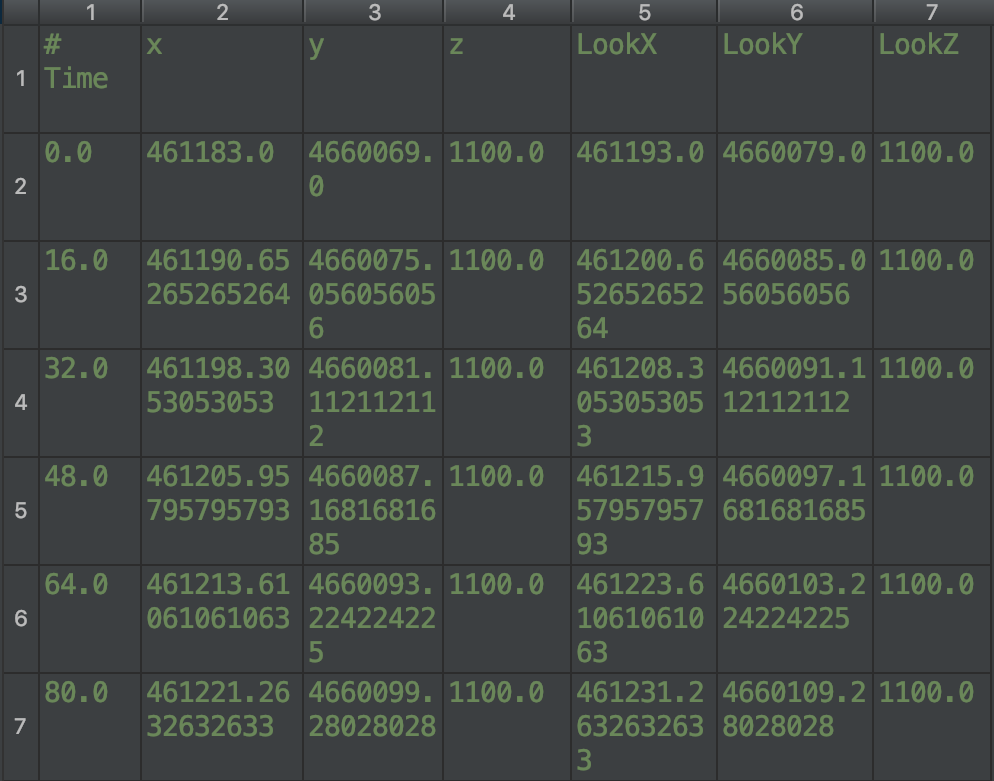
\includegraphics[width=0.45\textwidth]{fitxervehicle}
	\captionsetup{labelformat=empty}
	\caption{CSV file to control a vehicle}
	\label{fig-fitxervehicle}
\end{figure}


\begin{figure}[!h]
\centering
  	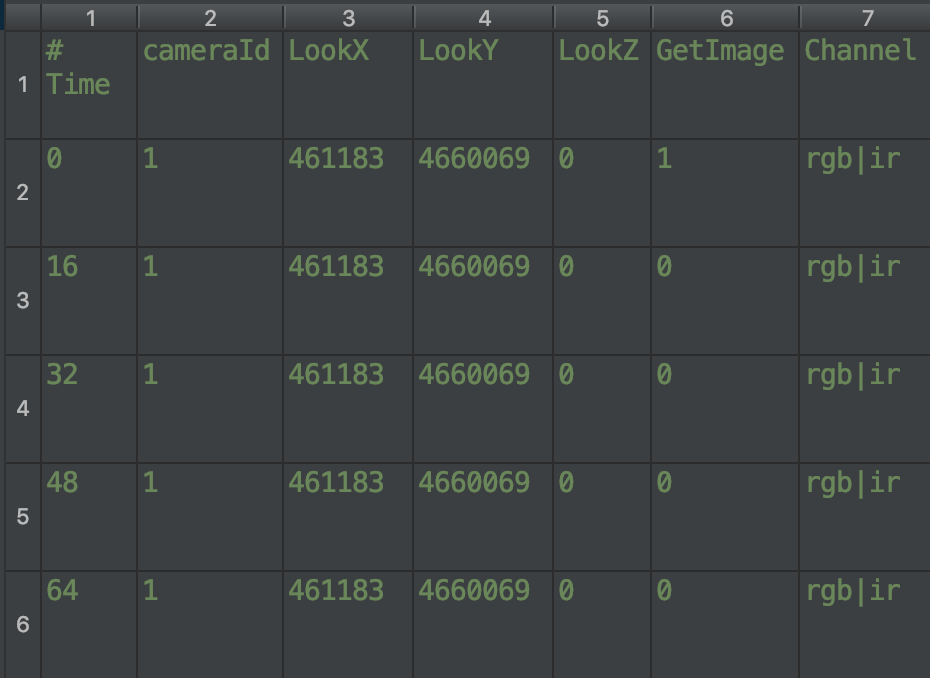
\includegraphics[width=0.45\textwidth]{fitxercameres}
  	\captionsetup{labelformat=empty}
	\caption{CSV file to control cameras}
	\label{fig-fitxercameres}
\end{figure}

\newpage
\subsection{Requirements to execute GEOTool}
\label{appendix:requirementsgeotool}

In order to use this application correctly we will have to have installed the Anaconda package (Tested with version 4.6.11 and Python 3.7.3) to which the 'utm' library will be installed with the command ''pip install utm''.

\subsection{Requirements to execute GEOControl}
\label{appendix:requirementsgeocontrol}

In order to use this application correctly we will have to have installed the Anaconda package (Tested with version 4.6.11 and Python 3.7.3) to which the ''mprpc'' library will be installed with the command ''pip install mprpc''.


\end{document}

